\documentclass[12pt]{article}

% Packages
\usepackage{hyperref}
\usepackage{physics}
\usepackage{amsmath}
\usepackage{indentfirst}
\usepackage{mathtools}
\usepackage{graphicx}
\usepackage[super]{natbib}
%\usepackage[super]{bib}
\usepackage[margin=0.75in]{geometry}
% End Packages

% Shortcuts
\newcommand{\schr}{Schr\"odinger}
\newcommand{\xhat}{\hat{\textbf{x}}}
\newcommand{\yhat}{\hat{\textbf{y}}}
% End Shortcuts

% Images Path
\graphicspath{ {images/} }
% End Images Path

\begin{document}
\title{A Review of Basic Quantum Mechanics Applied to Optical Pumping}
\author{Karl Ahrendsen}
\maketitle{}

\section{Introduction}
In Atomic, Molecular,
and Optical Physics, a topic of interest is the collisions between
basic 
objects, such as atoms, molecules, and elementary particles.
Our research group is focused on the study of spin-polarized electrons. 
An electron beam can be easily created and collided
with objects of interest,
but this is not the most simplified interaction
which can occur, as electrons also have spin, which can distinguish one 
electron from another. We are interested in obtaining a source which
outputs electrons of only one polarization, referred to as a spin
polarized electron source.

Our research group has created a source of spin polarized
electrons using spin-exchange interactions with the alkali metal
rubidium~\cite{rbSource}.  Our current method of obtaining 
polarized electrons involves optically pumping a rubidium vapor
with circularly polarized light. Then an unpolarized electron beam
is passed along the same path of the light 
through the polarized vapor. Spin exchange interactions
transfer the spin of the rubidium vapor to the electrons, and the 
result is a polarized electron beam. This approach makes intuitive
sense; circularly polarized light goes in and the circular
nature of the light causes things to start spinning.

Another research group in Wisconsin polarizes their alkali metal
in a different manner~\cite{swenson}. They pump their alkali metal, 
potassium, with
\emph{linearly} polarized light, perpendicular to the direction
of propagation of the electrons. The result is the same, a collection
of spin polarized alkali metal atoms, which could be used to create
a spin polarized electron beam. This approach is less intuitive
because the light we are pumping with does not have an rotation 
associate with it.

The goal of this paper is to thoroughly
explain how both of these approaches achieve a circularly polarized
alkali metal vapor, as well 
as to examine the feasibility of using linearly polarized light
for polarization in our own apparatus.

This goal will  be accomplished by first explaining the basics 
of atomic physics for pumping alkali atoms, including notation, energy
levels, angular momentum, and selection rules. After this we
will examine how our description of the energy changes in the
presence of a magnetic
field. Once these basics of pumping have been established we will
examine the specific case of transverse optical pumping. 

\section{Basics of Energy Levels of Alkali Atoms}
The process of optically pumping a gas refers to the 
act of moving a collection of atoms into the 
same energy state. As a mechanical analogy, one could
imagine that we have a bucket of atoms. The bucket 
represents the energy level that the atoms
occupy. We could put a hose into this
bucket and take some of the atoms from one bucket and
place them in another. In optical pumping, the role of 
this pump is played by the laser. 

To be able to understand how optical pumping works a firm 
understanding of the quantum mechanics involved in this 
process is needed. For this reason, I begin with a review of the energy
levels of an atom. For the sake of simplicity, I will complete
this discussion using
Hydrogen as the example atom, but the equations may be 
easily adjusted to be appropriate for an alkali atom.
These modifications will be discussed in Sections \ref{energyLevels}
and \ref{angularMomentum}. Throughout this discussion
the system of Gaussian units will be used. 
	\subsection{No Magnetic Field}
    We begin describing the energy levels in the absence of 
    a magnetic field. This consists of a slow buildup 
    from the Schr\"odinger equation starting with the radial
    equation and then adding in the orbital part. Intrinsic 
    angular momentum is introduced here before moving on to
    the selection rules which govern acceptable transitions
    between states. This is intended to be a swift tour through
	many main results of Quantum Mechanics relevant to 
	Optical pumping. If the reader is not familiar with the 
	concepts, any elementary quantum mechanics textbook
	such as Shankar~\cite{shankar} could be used to alleviate confusion.
		\subsubsection{Radial Solution Energy Levels}\label{energyLevels}
		The energy levels for hydrogen are found by solving the
		{\schr} equation with $V=-e^2/r$. 

		\begin{equation}
		  H\psi = E\psi
		\end{equation}
		where the Hamiltonian $H$ is 
		\begin{equation}
			H=-\frac{d^2}{dr^2}-\frac{2m}{\hbar}\Big[-\frac{e^2}{r} + \frac{l(l+1)\hbar^2}{2mr^2}\Big]
		\end{equation}
		
		Since this is a spherically
		symmetric potential, the Hamiltonian and angular momentum
		operators commute and we can split the wave function into a
		radial part and an angular part. 
		\begin{equation}
			\psi(r,\theta,\phi)=R(r)Y(\theta,\phi)
		\end{equation}

		By examining only the radial part, we find that the energies
		are quantized and correspond to the values:
		\begin{equation}\label{energyLevelsEq}
			E_n=\frac{-me^4}{2\hbar^2n^2},\quad n=1,2,3,...
		\end{equation}

		The result from quantum mechanics that the energy levels 
		of the hydrogen atom are 
		quantized is of central importance to optical pumping. 
		Each energy level from the equation above 
		corresponds to a certain configuration of the 
		atom, or a state. If the atom starts in one state, it can 
		transition to another, but
		only if a special set of rules is fulfilled. 
        For our description so far, there is only one rule;
		whatever the difference between the energy levels is, 
		an equal amount must be input into the atom from an outside
		source. For optical pumping, this outside source
		is the electromagnetic radiation from the pumping laser.
	
        More of these rules will appear as we
        expand our description of the hydrogen atom.
        In general, these restrictions 
        are called selection rules and will be further
        discussed in 
        Section \ref{selectionRules}.

        In order to more conveniently describe 
        this process of transitioning from one state to another
        we will introduce Dirac Bra-Ket notation. In 
        Bra-Ket notation a state is identified by 
        either a ``bra" $\bra{n}$
        or a ``ket" $\ket{n}$. Here, $n$ is a quantum number
		which indicates the excitation level of the state.
		It is the same $n$ which is seen in Eq.(\ref{energyLevels}). 
		In our simplistic description thus far, 
		this is all we need to describe the state.
		As we add in more detailed descriptions of 
		the state, we will require additional quantum
		numbers to completely 
		describe the state.

		The transition from one state to another in optical pumping
		will occur because of laser light incident on the electron.
		To account for this additional energy added into the system 
		we must augment
		our previous Hamiltonian. We call the Hamiltonian without 
		the energy from the light the unperturbed Hamiltonian and 
		give it the variable name $H_o$.
		\begin{equation}
			H_o=-\frac{d^2}{dr^2}-\frac{2m}{\hbar}\Big[-\frac{e^2}{r} + \frac{l(l+1)\hbar^2}{2mr^2}\Big]
		\end{equation}
		The energy from the light is called a perturbation and we
		can write its contribution to the atom as 
		\begin{equation}
			H_1=\frac{e}{2mc} \vec{A_o} \cdotp \vec{P}
		\end{equation}

		In the above expression, $e$ , $m$, and $p$ represent the charge, mass,
		and momentum of the electron, respectively. The variable $c$ represents
		the speed of light and $\vec{A_o}$ represents the time-independent 
		vector potential ($\vec{A}(t)=\vec{A_o}e^{-i\omega t}$). 
		Here we are leaving out the derivation of this term and
		its time dependence because they will not be directly 
		relevant to our discussion of optical pumping. Additionally, 
		we have taken the electric dipole approximation to simplify
		the discussion. 
		The interested reader should
		consult other texts, such as Shankar, for further information about the 
		perturbation and the approximation we make here. 

        Though we provided this specific example of the perturbing 
        Hamiltonian being electromagnetic radiation, we will also 
        describe other shifts in the energy within this same framework,
        namely the magnetic field.

		Before continuing on to a discussion of angular momentum, 
		we will begin our discussion of how the alkali metals differ
		from hydrogen. The alkali metals occupy the left-most
		column in the periodic table (Fig. \ref{periodicTable}), 
		indicating that they have one
		electron in their outermost energy level, a valence electron,
		and all energy sub-levels filled. 
		\begin{figure}[ht]
			\centering
			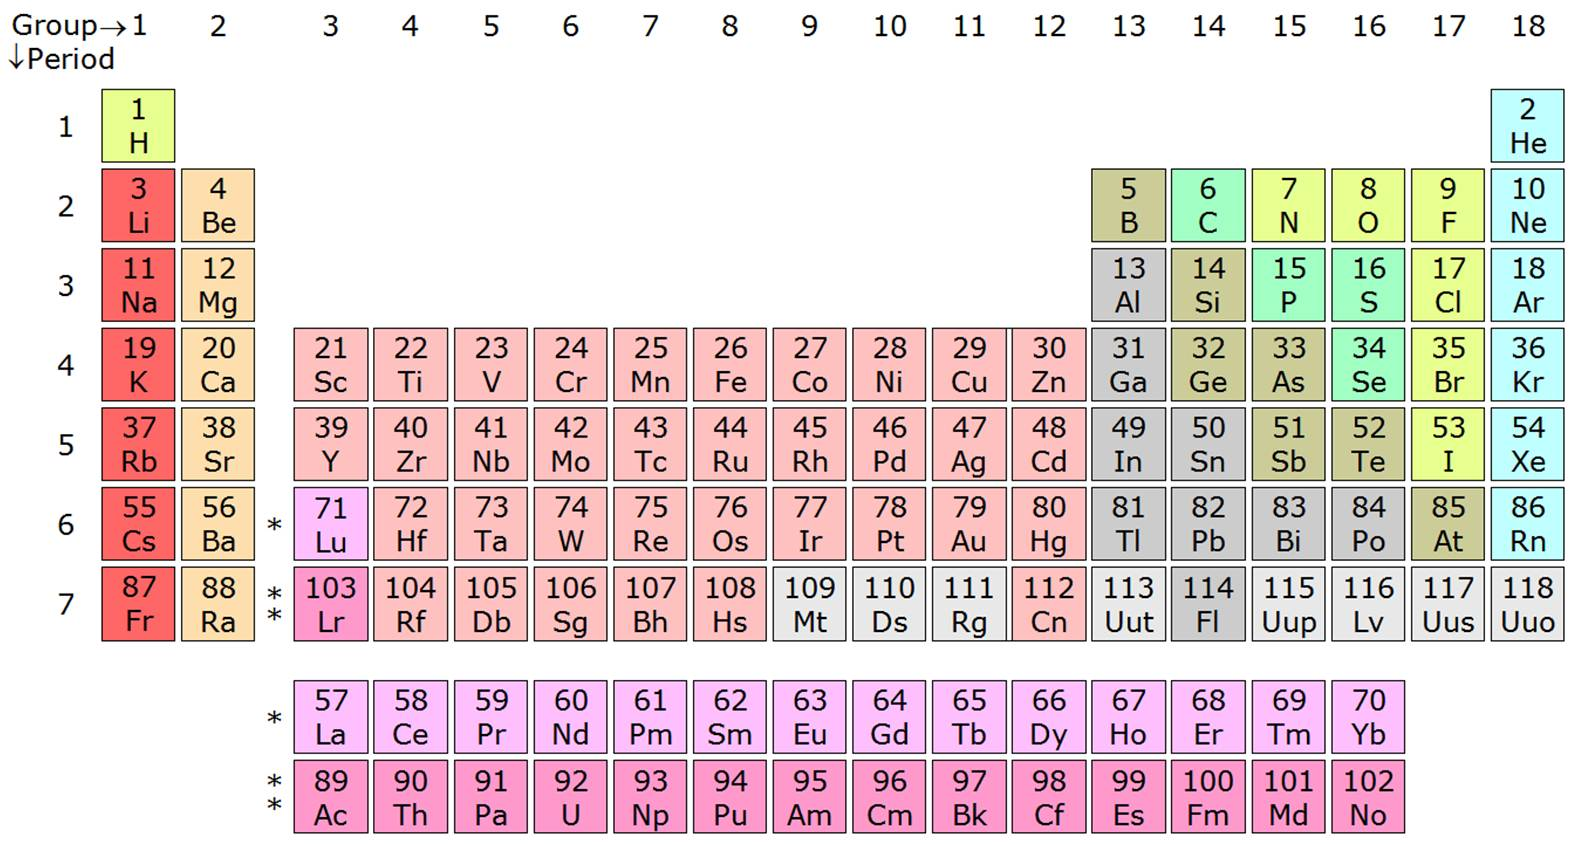
\includegraphics[width=\textwidth]{periodicTable}
			\caption{\label{periodicTable}The periodic table 
				of elements. The alkali metals 
			are in group 1 and indicated by the red boxes. Image
			used under creative commons license and obtained
			from Wikipedia~\cite{periodicWiki}.}
		\end{figure}
		The lower energy level
		electrons screen the charge of the nucleus, leaving the effective
		charge that the valence electron experiences 
        a single elementary charge. The connection between the alkalis
		and Hydrogen is then apparent, hydrogen is a single negative charge
		orbiting a single positive charge and the alkalis are a single
		negative charge orbiting a combination of charges which 
		can be approximated to be a single positive charge.
        Because the lower energy level electrons do not always completely
		mask the charges in the nucleus, the energy level equation 
		needs to be modified. A common
        expression for the modified energies is

		\begin{equation}\label{modEnergy}
            E_n=\frac{-me^4}{2\hbar^2(n-\delta(l))^2},\quad n=1,2,3,...
		\end{equation}

        Here $\delta$ is a function called the quantum defect which
        depends on the quantum number $l$, representing angular momentum.
        Angular momentum is the subject of the next section, and we 
        will discuss this dependence further in that section.

		\subsubsection{Angular Momentum}\label{angularMomentum}
		There are many aspects of angular momentum to consider
		in pumping. First, we discuss the orbital angular momentum of 
		the electron. Then, we will introduce intrinsic angular momentum,
		or spin, of the electron. After this, we will continue in the 
		intrinsic realm with the angular momentum of the nucleus of 
		the atom. A brief discussion of photon angular momentum will
		close out the section.

        Previously, we arrived at our solution for the electron energy 
		levels
        of hydrogen by just considering the radial part of the
        equation. We will now discuss the important concepts related
        to the angular part of the solution. 
        
        Like the radial part, 
        we also find out that the angular part has solutions that 
        are quantized. We denote these discrete values that a state
		can occupy by the quantum number $l$. This value serves as an
		indication to the amount of orbital angular momentum that the 
		system has. A natural assumption might then be that
		the energy equation would have $l$ dependence; if 
		something is orbiting ``more" (has a higher value 
		of $l$) it should have more energy. This, however is not
		the case for hydrogen. The quantum number $l$ has no effect on the 
		energy of the system. Whenever a quantum number does not
		have an effect on the energy of the system, it is said to
		be degenerate. The source of this degeneracy is sometimes said 
		to be ``accidental," but in reality stems from 
		the conservation of the Runge-Lenz vector.

		The alkali metals, on the other hand, do change energy levels with
		increasing $l$. This can be seen in Eq. (\ref{modEnergy}) where 
		the quantum defect
		is subtracted from the denominator, making the term larger and the
		energy more negative.
		This difference is most pronounced for \emph{low} values 
		of $l$, and once the electron reaches the d orbital the difference
		all but disappears. In our application of optical pumping,
		we focus on this difference between different levels of $l$,
		often pumping between these states.
		
		Whether hydrogen or alkali metal, the allowed 
		values of $l$ are determined when solving
		the radial energy equation. We find that

		\begin{equation}
			l=n-k-1,\quad k=0,1,2,3,...,n
		\end{equation}

		so $l$ has a maximum value of $n-1$. To aid in making
		these orbitals easier to discuss, we introduce 
		spectroscopic notation which is commonly used in the 
		literature. In this notation
		each value of $l$ is associated with a letter to indicate
		the shape of the atomic orbitals. When $l=0$, we name the 
		orbital shape s. As $l$ increases, the subsequent orbitals
		are named: p,d,f,g,h... We will only deal with the s and p 
		states in our discussion here. 

		In this notation, the letter indicating the orbital 
		and the number representing the principal quantum number 
		are often combined, such that the state of the atom 
		is described by $nl$, where $n$
		represents the energy level and $l$ represents the orbital
		occupied. For example, if the electron is in the 4th energy
		level and has 0 angular momentum, we would say that it is
		an electron in the 4s state. We will return to augment this 
		notation after introducing the electron's intrinsic angular
		momentum.

		The quantum number $l$ is associated with orbital momentum 
		which is a vector quantity. Because of this, knowing $l$
		does not tell us the full story. 
		There is another quantum number, $m$, which is associated 
		with the angular momentum $l$. This value serves to indicate
		how much of the angular momentum is spinning in a arbitrarily
		chosen direction. Another term we will use to refer to this
		is the projection it has in the given direction.
		Most commonly, this direction is chosen
		to be in the $z$ direction. We again find that the quantum
        number $z$ has no effect on the angular momentum. This result
        is perhaps easier to identify, as the energy of something 
        orbiting in one direction should be the same as the energy 
        of the same thing orbiting in another. The values that the 
		quantum number $m$ can hold are of course
		closely related to $l$. They range from $+j$ to $-j$ in
		integer steps. 

        The independence of the energy levels from $m$ is only true
        if the electron is a spin-less particle. It is a well known
        fact, however, that the electron does possess an intrinsic 
        angular momentum or ``spin." We will come to a discussion of 
        how this contributes to the energy levels in a moment, but 
        for now, simply note that the electron has an angular 
        momentum associated with it. The quantum number associated
        with this angular momentum is $s$. It is a vector 
		quantity, and the values it can take are $+1/2$ and $-1/2$.
		Because spin is also a vector quantity, we have 
		yet another quantum number $m$ to describe the projection 
		of $s$ in a given direction. In most cases, the angular
		momentum that $m$ is associated with will be clear. If
		there is ever a chance of confusion, the ``spin" $m$ is
		given a subscript $s$ so it is indicated by $m_s$.

        These angular momentum variables associated with the
        electron are often combined to simplify notation. We
        introduce a new quantum number $j$ which is equal to
        the vector sum of the orbital angular momentum of the
        electron with the spin angular momentum of the electron,
        like so: 

        \begin{equation}
            \vec{J} = \vec{L} + \vec{S}
        \end{equation}

        Now that we have discussed spin, we need to modify our 
        spectroscopic notation of the atomic states to include
        this information. There are three changes that need to 
		be made. First, the lowercase letters are changed to
		uppercase letters. Second, we now include a subscript after
        the atomic orbital letter to indicate the total angular
        momentum ($\vert\vec{J}\vert$) of that state. 
		Third, we append a superscript $2s+1$ to the left of
		the atomic orbital letter to indicate the number of
		spin projections available. In general
		this means the state we be noted as $n\prescript{2s+1}{}l_{J}$. For 
		a specific example, 
        a spin up electron ($s=1/2$) in the $n=4$ state with 
        0 orbital angular momentum ($l=0$ , $j=1/2$) would be 
        described by $4\prescript{2}{}S_{1/2}$.

		We also take a moment here to revisit bra-ket notation.
		Each of the quantum numbers we have introduced serves
		to identify the state which an electron in an atom 
		currently occupies. We therefore include them, along with
		$n$, inside our bra-kets. We can fully describe a state by
		$\ket{nlmsm_s}$, but it is also common to just focus on
		the total angular momentum $j$, and write $\ket{njm}$ to
		describe the state.

        The electron is not the only particle with an intrinsic
        angular momentum. Protons and neutrons have it as well,
        meaning the nucleus of our atom will also have a
        spin which will contribute to the energy. The variable
        associated with nuclear angular momentum is $I$ and
        for the most common isotope of potassium, its values
        range between $+4$ and $-4$ in integer steps. 
	
		This completes our discussion of the angular momentum
		of the atom, but our discussion of angular momentum in 
		general would not be complete without mentioning light.
		Photons are known to have spin and can thus carry 
		angular momentum as well. Though photons are mentioned
		here to introduce source of the angular momentum,
		we will primarily deal with
		electromagnetic radiation in the macroscopic sense, 
		that is to say, with the electric field. Here, we 
		observe angular momentum in the polarization of 
		electromagnetic radiation. If an electric field has
		circular polarization in the z-direction, we can 
		describe it as:

		\begin{equation}\label{circleLight}
			\vec{E}=-E_o \xhat  +iE_o \yhat 
		\end{equation}

		We will refer to this circularly polarized light as 
		$\sigma^{+}$ or $\sigma^{-}$ light for right and 
		left handed polarizations respectively.
		
		\subsubsection{Selection Rules}\label{selectionRules}
		We mentioned in Section \ref{energyLevels} that there
		were selection rules between energy levels of an atom.
		These selection rules arise because of the requirement
		of conservation of energy. We also know that angular 
		momentum must be conserved, so we also have selection
		rules related to the angular momentum in a system. 

		To more easily describe these selection rules, it is
		convenient to introduce irreducible tensor operators. 
		Irreducible tensor operators provide concise information
		about the angular momentum contained in an operator.
		The operator is written in the form $T^{q}_{k}$ where
		$k$ represents the angular momentum of the operator
		and $q$ represents the projection of angular momentum
		along the $z$ axis contained by the operator. When a
		irreducible tensor acts on a state, it adds $k$ and 
		$q$ angular momentum to that state. The angular momentum
		of the initial state plus the operator must be
		equal to the angular momentum of the final state. In
		terms of an equation, we write this as: 

		\begin{equation}
			\bra{\alpha'j'm'}T^{q}_{k}\ket{\alpha jm}=0\quad \textrm{unless} \quad k+j\geq j' 
			\geq \vert k-j \vert,\quad m'=m+q
		\end{equation}

		How do we write the electric field (our most common
		operator on the state) in terms of an irreducible 
		tensor? The irreducible tensor notation of the 
		electric field is equal to a linear combination of
		the vector components. This relationship is as 
		follows:

		%\begin{equation}
			\begin{gather}
			T^{\pm1}_1 = \mp \frac{V_x \pm iV_y}{2^{1/2}} \equiv V^{\pm1}_{1} 
			\\
			T^{0}_1 = V_z \equiv V^{0}_{1} 
			\end{gather}
		%\end{equation}

		Therefore our electric field in Eq. (\ref{circleLight}) can
		be written in irreducible tensor form as $E^{1}_1$ and 
		would modify both the $j$ and $m$ 
		quantum numbers.
\subsection{With Magnetic Field}
	In the presence of a magnetic field, our energy levels will be modified.
	The magnetic moment from the spin of the electron will interact
	with the field, and one spin direction will have a 
	higher energy than the other. These effects are
	visible even before applying an external 
	magnetic field. To see how this arises, 
	consider the orbiting electron
	when viewed in its own rest frame. From this
	perspective the  
	proton is orbiting it. Moving charges
	are currents, so the proton creates a
	magnetic field with which the spin of the electron 
	interacts. This interaction between the spin of the 
	electron and the proton's "current" will cause
	the energy of the electron to be different depending
	on the orientation of its spin. This difference is 
	important because otherwise there would be no 
	selection rule to distinguish
	between a $4\prescript{2}{}P_{1/2}$ with 
	$m_s=1/2$ and $4\prescript{2}{}P_{1/2}$ with $m_s=-1/2$.
	Because of this difference in energies, called 
	fine-structure, we can isolate transistions to take
	the electron to a specific spin state.

%	\subsection{Weak Magnetic Field}
%		\subsubsection{Energy Levels}
%		\subsubsection{Coupling}
%		\subsubsection{Selection Rules}
%
%	\subsection{Strong Magnetic Field}
%		Energy splitting due to fine structure?
%		Energy splitting due to hyper-fine structure?

\section{Longitudinal Optical Pumping}
To describe the longitudinal optical pumping, I will
first describe the physical components necessary for
obtaining a polarized alkali metal vapor. After these 
components have been established a discussion of the 
allowed transitions in the alkali atom will follow. 
	\subsection{Required Setup}
    Longitudinal optical pumping, the way our apparatus is 
    currently configured, requires a magnetic field and
    circularly polarized light. The magnetic field
	serves mainly to preserve the spin of the alkali
	atoms over time. If the magnetic field were not 
	present, the atoms would precess around whatever
	residual magnetic field exists within the vicinity
	of the apparatus and no longer be coherently pointing
	in one direction. The circularly polarized light
	is what allows us to orient the spins of the alkali
	atoms in the same direction. We can choose either 
	$\sigma^{+}$ or $\sigma^{-}$ for this, but for 
	definiteness, let us choose $\sigma^{+}$

	\subsection{Allowed Transitions}
	The electrons in the potassium will start in the ground
	state and be randomly oriented either up or down.
	Both of these states are described by 
	$4\prescript{2}{}S_{1/2}$.
	Which states they can transition, or be pumped to, 
	will be determined by the selection
	rules for the interaction. Since we are pumping with
	circularly polarized light, our electric field vector
	will have a real part and an imaginary part:
	
	\begin{equation}
		\vec{E}=E_o \xhat  -iE_o \yhat 
	\end{equation}

	Putting this into irreducible tensor form, we have 

	\begin{equation}
		\vec{E} \rightarrow E_{1}^1
	\end{equation}

	which will impart one vector unit of $l$ angular momentum,
	and subract unit of $m$ angular momentum. Therefore, if
	our initial state is $\ket{njm}$ our final state must
	be $\ket{n(j\pm1)(m-1)}$. 	

	In the literature, this is more
	commonly described in spectroscopic notation. If we begin 
	with a spin-down electron, we would have the transisition
	$4\prescript{2}{}S_{1/2} \rightarrow 4\prescript{2}{}P_{3/2}$
	for our electron.
	On the other hand, if we began with a spin-up electron, we 
	would get 
	$4\prescript{2}{}S_{1/2} \rightarrow 4\prescript{2}{}P_{1/2}$
	for our electron transistion. Fine structure splitting 
	allows us to tune our laser to a frequency that matches 
	the energy difference of only one of these transistions. 
	Again, the choice is arbitrary, but for definiteness let us
	choose the second of these transistions. 

	After being excited, the electron will eventually decay
	down to the ground state. When it does this, it can go to
	either the spin-up ground state or the spin-down ground
	state. These transistions do not have equal probability,
	however, with the decay to the spin-up state being twice 
	as likely~\cite{swenson}. 

	The electrons that are in the spin-down state will remain
	there, because there is no light incident on the system to 
	excite them out of their ground state. The electrons that 
	return to the spin-up state will again go through the same 
	pumping process until they decay to the spin-down state.
	By this process, we then create a population of spin-down
	electrons. The electrons exchange their spin with 
	the nucleus, thereby giving a collection of spin-polarized
	potassium atoms. 

\section{Transverse Optical Pumping}
To describe transverse optical pumping, we will compare it to 
linear pumping and identify the similarities and differences.
	\subsection{Required Setup}
	The required setup for transverse pumping also requires
	a magnetic field for the same reasons as previously indicated
	but this time linearly polarized light is necessary.
	Furthermore, the polarization direction of the light
	must be aligned to be parallel with the magnetic field
	used to preserve the spins. For concreteness we assume
	that the magnetic field is oriented in the z-direction.

	\subsection{Allowed Transitions}


\section{Conclusion}

\bibliographystyle{plain}
\bibliography{bibPotassium}

\end{document}
